\documentclass[border=4pt]{standalone}
\usepackage{tikz}
\usepackage{pgfplots}
\pgfplotsset{compat=1.18}
\usetikzlibrary{shapes.geometric,arrows.meta,positioning,fit,calc,decorations.pathreplacing}
\usepackage{xcolor}
\definecolor{bestcol}{HTML}{1565C0}
\definecolor{freegreen}{HTML}{2E7D32}
\definecolor{learnblue}{HTML}{1565C0}
\definecolor{fusred}{HTML}{C62828}
\newcommand{\best}[1]{{\color{bestcol}\textbf{#1}}}
\begin{document}
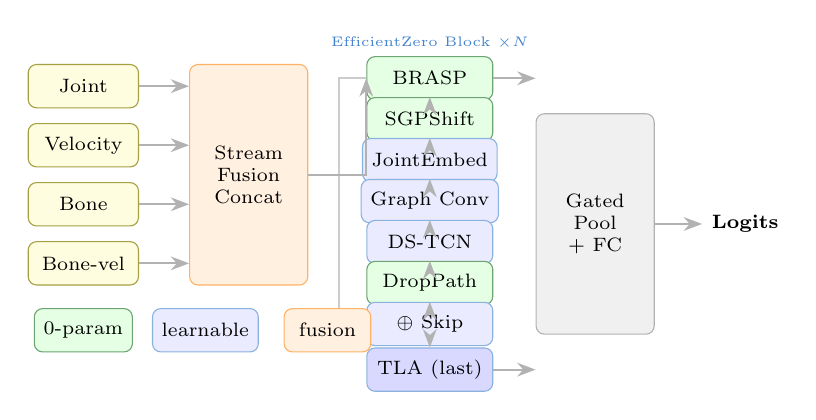
\begin{tikzpicture}[
  every node/.style={font=\scriptsize},
  box/.style={draw, rounded corners=3pt, minimum width=1.6cm,
              minimum height=0.55cm, align=center, fill=white},
  free/.style={box, fill=green!10, draw=freegreen!70},
  learn/.style={box, fill=blue!8, draw=learnblue!50},
  stem/.style={box, fill=orange!12, draw=orange!60},
  cls/.style={box, fill=gray!12, draw=gray!60},
  inp/.style={box, fill=yellow!12, draw=yellow!60!black, minimum width=1.4cm},
  arr/.style={-Stealth, thick, draw=gray!60}
]

%% input streams
\node[inp] (xj)  at (0, 0)    {Joint};
\node[inp]  (xv)  at (0,-0.75) {Velocity};
\node[inp]  (xb)  at (0,-1.50) {Bone};
\node[inp]  (xbv) at (0,-2.25) {Bone-vel};

%% stem
\node[stem, minimum height=2.8cm, minimum width=1.5cm]
  (sfuse) at (2.1, -1.125) {Stream\\Fusion\\Concat};

\foreach \s in {xj,xv,xb,xbv}
  \draw[arr] (\s.east) -- (\s.east -| sfuse.west);

%% block internals (stacked, right of stem)
\node[free]  (brasp) at (4.4,  0.10)  {BRASP};
\node[free]  (sgp)   at (4.4, -0.42)  {SGPShift};
\node[learn] (je)    at (4.4, -0.94)  {JointEmbed};
\node[learn] (gcn)   at (4.4, -1.46)  {Graph Conv};
\node[learn] (tcn)   at (4.4, -1.98)  {DS-TCN};
\node[free]  (dp)    at (4.4, -2.50)  {DropPath};
\node[learn] (res)   at (4.4, -3.02)  {$\oplus$ Skip};

% skip bypass
\draw[arr, gray!40]
  (brasp.west) -- +(-0.35,0) |- (res.west);

\draw[arr] (sfuse.east) -- (brasp.west |- sfuse.east)
  -- (brasp.west);
\foreach \a/\b in {brasp/sgp, sgp/je, je/gcn, gcn/tcn, tcn/dp, dp/res}
  \draw[arr] (\a)--(\b);

\node[font=\tiny, text=learnblue!80] at (4.4, 0.55) {EfficientZero Block $\times N$};

%% TLA
\node[learn, fill=blue!15] (tla) at (4.4, -3.60) {TLA (last)};
\draw[arr] (res)--(tla);

%% classifier
\node[cls, minimum height=2.8cm, minimum width=1.5cm]
  (pool) at (6.5, -1.75) {Gated\\Pool\\+ FC};
\draw[arr] (tla.east)  -- (tla.east  -| pool.west);
\draw[arr] (brasp.east) -- (brasp.east -| pool.west);

%% output
\node[right=0.6cm of pool] (out) {\textbf{Logits}};
\draw[arr] (pool)--(out);

%% legend
\node[free,  minimum width=1.1cm] at (0,-3.10) {0-param};
\node[learn, minimum width=1.1cm] at (1.55,-3.10) {learnable};
\node[stem,  minimum width=1.1cm] at (3.1,-3.10) {fusion};

\end{tikzpicture}
\end{document}
